\documentclass{article}

% if you need to pass options to natbib, use, e.g.:
%     \PassOptionsToPackage{numbers, compress}{natbib}
% before loading neurips_2018

% ready for submission
% \usepackage{neurips_2018}

% to compile a preprint version, e.g., for submission to arXiv, add add the
% [preprint] option:
%     \usepackage[preprint]{neurips_2018}

% to compile a camera-ready version, add the [final] option, e.g.:
\usepackage[preprint]{style}
\usepackage{xcolor}
\usepackage{graphicx}


% to avoid loading the natbib package, add option nonatbib:
%     \usepackage[nonatbib]{neurips_2018}

\usepackage[utf8]{inputenc} % allow utf-8 input
\usepackage[T1]{fontenc}    % use 8-bit T1 fonts
\usepackage{hyperref}       % hyperlinks
\usepackage{url}            % simple URL typesetting
\usepackage{booktabs}       % professional-quality tables
\usepackage{amsfonts}       % blackboard math symbols
\usepackage{nicefrac}       % compact symbols for 1/2, etc.
\usepackage{microtype}      % microtypography
\usepackage{caption}
\usepackage{subcaption}
\usepackage{multirow}
\usepackage{booktabs}


% draft of title 
\title{Reimplementation of Self-Classifier on new datasets
}

% The \author macro works with any number of authors. There are two commands
% used to separate the names and addresses of multiple authors: \And and \AND.
%
% Using \And between authors leaves it to LaTeX to determine where to break the
% lines. Using \AND forces a line break at that point. So, if LaTeX puts 3 of 4
% authors names on the first line, and the last on the second line, try using
% \AND instead of \And before the third author name.

\author{
    Shaochen Bai        \\ \texttt{shaochen@kth.se} \And 
    David Bardvall      \\ \texttt{bardvall@kth.se} \And 
    Riccardo Periotto   \\ \texttt{periotto@kth.se}
}

\begin{document}
% \nipsfinalcopy is no longer used

\maketitle

\begin{abstract}
% Give an overview of what you have done in the project with the key results and findings of your work. Should be no more than 300 words.
In this work, we re-implement  "Self-Classifier" \cite{self_classifier}, a novel self-supervised end-to-end classification learning approach presented in ECCV 2022. In addition to achieving better performance than its competitors over the self-supervised challenges, the approach guarantees important properties such as scalability, single-stage end-to-end training, and non-degenerate solution. 
We apply the proposed method to MNIST, CIFAR-10, CIFAR-20, and STL-10 in the evaluation of unsupervised clustering performance. Standard linear probing experiments and ablation studies are run to examine different aspects of the model. We also extend the visualization section to analyze the representation learning quality and prior enforcement situation.
Although the mathematical formulations of the model as well as its implementation details are mostly covered in the original paper, additional code resources are referred to set the hyperparameters properly. 
Our code is available on KTH GitHub: \footnote{https://github.com/riccardoperiotto/KTH-DD2412-DeepLearningAdvanced}.  \\

\textbf{Keywords}: Self-Supervised Learning, Representation Learning, Clustering, Non-contrastive Learning
  
\end{abstract}



\section{Introduction}
% Describe the problem, the approach of the paper, the experiments, and the results. At the high-level talk about what you worked on in your project and why it is important. Then give an overview of your results. 
% + code repository
Many of the most significant results achieved so far by deep learning algorithms come from supervised settings with access to large amounts of labeled data.
Such large-scale labeled datasets are not always guaranteed, especially in the field where human labeling is expensive or restricted (medical field for example).
On the other hand, with the development of big data, unlabeled data are easier to obtain through the Internet more than ever, and the idea of unsupervised learning is to train the model without supervised knowledge but achieve rather competitive performance nonetheless. The label-free technique greatly expands the possible application fields of deep learning and increases its influence in every modern industry.


There are many subcategories in the field of unsupervised learning, and the proposed paper\cite{self_classifier} focuses on self-supervised learning aiming to train the model to obtain high-level natural features in the data by solving one or a set of pretext tasks.
After learning to recognize these features, the model can either be used directly for representation retrieving or fine-tuned to solve task-specific downstream tasks \cite{self_classifier}\cite{swav} \cite{simsiam}\cite{byol}. 
The main focus of the literature on self-supervised learning is to understand and develop the most suitable pretext tasks for some specific target tasks. At the moment, contrastive learning is the pretext task defining the state-of-the-art results \cite{byol}\cite{simclr}, the idea of which is to train the model to predict the similarity (or the distance) between two augmented inputs. 
However, current contrastive learning methods are prone to degenerate solutions, where the models map all the inputs into a single representation. 
Targeting the problem, the paper proposed a loss function that enforces a uniform prior to all the classes during training which avoids the pitfall and learns to cluster data concurrently. From a general perspective, the prominent characteristics of Self-Classifier also include its strong performance, high scalability, and simple single-stage end-to-end training structure. 

\textbf{The main contributions of our work are that:}

$\bullet$  We implement and compare Self-Classifier with its competitors on smaller datasets CIFAR10, CIFAR20, MNIST, and STL10;

$\bullet$  We broadly study the related literature and conclude the main differences;

$\bullet$ Extensive visualization and ablation study are run to deepen our understanding of the model.

\section{Related Work}
\label{sec:related_work}
%Discuss the published work related to your project paper, the types of experiments you do and the additional method that you have added to this work or you have compared this paper with (if any).
% In the section, we cover the pretext task of contrastive learning and their performance in downstream tasks mainly deep clustering.

\subsection{Contrastive Learning}
It is well worth noticing that contrastive learning is just one of the proposed pretext tasks for self-supervised learning. Outside of this category, many non-contrastive tasks have also demonstrated their validity,  some of the most popular among which include colorization, jigsaw puzzle, image inpainting, relative patch prediction, context prediction, and rotation prediction\cite{self_classifier}\cite{byol}. 
The key difference between contrastive and non-contrastive learning lies in the self-generated label that the model aims to predict. In non-contrastive learning, labels correspond to the augmentation applied to the inputs by the model. While in contrastive learning, labels act as a distance metric between the model's predictions of two different input augmentations. The goal here is to train the model to learn a feature representation that maximizes the distances between augmentation of different inputs and minimizes those between augmentations of the same data point \cite{byol}. 

Within the specific category of contrastive learning, there is an additional distinction between models trained with negative and positive pairs and those trained using only the positive ones. 
While both methods can successfully be trained to obtain optimal results \cite{simclr}, the underlying pretext task can sometimes be non-aligned with the downstream one, as described in \cite{self_classifier}. Also as negative samples act as a means to avoid degenerate solutions, models training only on positive pairs are more prone to the problem and additional care needs to be taken. 

% NEED TO CUT SOMETHING UNFORTUNATELY % The last fundamental role in contrastive learning is played by augmentation. Most of the augmenting techniques employed by the models we compared resemble each other, but the original paper refers especially to the ones proposed in \cite{byol}. We present more details on this topic in the methods \autoref{subsec:implementation_details}.

\subsection{Downstream Tasks}
Depending on the learning goals of subsequent downstream tasks, we can split the compared methods into two categories: those that only aim to solve representation learning and those that combine, in some way, representation learning and clustering. We highlight that both categories can solve the two tasks because: (i) It is always possible to apply additional clustering on the features obtained from a model of the first category; (ii) It is always possible to access the most informative features by retrieving representations from the backbone of a second category model. 

Regarding the first category, earlier models include Exemplar CNN \cite{cnn} and Non-Parametric Instance Discrimination (NPID) \cite{npid}, which suffer limitations such as poor scalability and lack of consistency across representations stored in the memory bank \cite{self_classifier}. More recent methods belonging to the category are MoCo \cite{moco}, BOYL \cite{byol}, SimSiam \cite{simsiam} and DINO \cite{dino}, which all adopt certain stop gradient operations to avoid the degenerative solution, regarding which constitutes the key difference between them and Self-Classifier. We will discuss this point thoroughly in the next section (\autoref{sec:methods}).

The second category methods mostly include the alternative clustering phase along with the representation learning, which results in the earlier models such as DEC \cite{dec}, JULE \cite{jule} hard to be tested on a larger-scale dataset for their computation inefficiency. DeepCluster works better but still requires a costly clustering phase and specific precautions to avoid collapsing to trivial solutions \cite{byol}. More recent methods such as SwAV \cite{swav}, SeLa \cite{sela}, SCAN \cite{scan} and IIC \cite{iic} improves efficiency and stability at the same time, and are easier to compare with our model for their similar architecture. 

What all the modern models from both categories have in common is that they are trained using only positive pairs (except MoCo), which as anticipated, makes them all prone to the degenerative solution. The main differences they have from one another consist of the various strategies implemented to avoid this problem. As in \cite{deepcluster}, we underline that the existence of the degenerative solution is not specific to the unsupervised training, but it is common to any method that jointly learns a discriminative classifier and the labels. 

% NOT TRUE, Simsiam scalers: Another thing to mention is that, among the mentioned models, SCAN \cite{scan} and SeLa \cite{sela} are the only ones capable of scaling to large datasets such as ImageNet \cite{imagenet}.

\section{Methods}
\label{sec:methods}
%Describe the original paper's method to the extent that you would need to make your report and findings understandable. Otherwise, here you can describe other methods that you compare with or other methods that you apply on top of what you reimplemented. Here, you also try to justify any methodical modification or incremental changes that you have added to the original paper.It may be helpful to include figures, diagrams, or tables to describe your method or compare it with other methods.
Although the former section covers the literature in general, we would discuss the key design aspects in more detail, and demonstrate the method of Self-classifier by comparing it with related models with a clear focus on the similarities and differences in how they avoid the degenerate solution.

\subsection{Avoid the degenerate solution}
\label{subsec:degenerate_solution}
% In the following, we compare the techniques for avoiding the degenerate solution when training on positive pairs. In addition to rejecting those techniques based on negative pairs, we also discarded those involving pre-training, memory bank, features post-processing, and cluster reassignment. We did that because, as briefly described in \autoref{sec:related_work}, modern techniques demonstrated to be better.

For the self-supervised techniques that do not rely on negative samples, we split them into three categories, namely external clustering, momentum encoder, and non-collapsing function. Since the principle of avoiding the degenerate solution behind the first two categories is practically the same, we further identify them together as stop-gradient operations, whose distinguishment is where the stop operation is applied.

External clustering is employed in models that simultaneously learn how to represent and classify the data. We mention that the models solving these tasks together most similar to Self-Classifier are SwAV \cite{swav}, SeLa \cite{sela} and SCAN \cite{scan}. The difference between these three concerning external clustering is that SwAV and SeLa implement it online through a Sinkhorn-Knopp distance algorithm, while SCAN implements it separately using K-means \cite{self_classifier}. 

MoCo \cite{moco}, BYOL \cite{byol}, and DINO \cite{dino} do not have a clustering phase and the stop gradient operation is obtained through a second network called momentum encoder. This idea originates from MoCo \cite{moco}, but despite acting as a precursor, this model is slightly different from the others as its training phase employs both positive and negative pairs. SimSiam \cite{simsiam} is a step in the direction of simpler models and a better understanding of the principles of Siamese networks. It prevents the degenerate problem by applying a stop-grad operation on one of the augmented views. Differently from BYOL \cite{byol} and other models for representation learning, SimSiam directly shares the weights between the branches elaborating the two augmentations. The SimSiam paper states that the method can be thought of as “SimCLR without negative pairs” and “SwAV without online clustering” \cite{simsiam}.

The third category of non-collapsing function is the most related to the proposed work, which solves the degenerate problem by defining the loss function or the objective function that enforces the predicted class to be distributed more uniformly. The idea of Self-Classifier \cite{self_classifier} is very similar to the one proposed in IIC \cite{iic} as their main point is to define a function that prioritizes solutions where the samples are spread among the different classes. 
IIC does that by defining an objective function that maximizes the mutual information between the predictions of two augmented views of the same sample. 
The loss function proposed by Self-Classifier instead is equivalent to the cross-entropy classification loss under a uniform label prior, which guarantees a non-degenerate, uniformly distributed optimal solution as explained in the original paper \cite{self_classifier}.

% HAD TO CUT
% The idea of uniform partitions is not something new. For example, also SwAV and SeLa's papers claim that their models are constrained to find a "balanced partition for each batch" \cite{swav} and "an equipartition of the data" \cite{sela}. The novelty of Self-Classifier is its simplicity in achieving this property.

In \autoref{fig:1}, we further illustrate the comparison in \cite{simsiam} with the models we described so far.

\begin{figure}
    \centering
     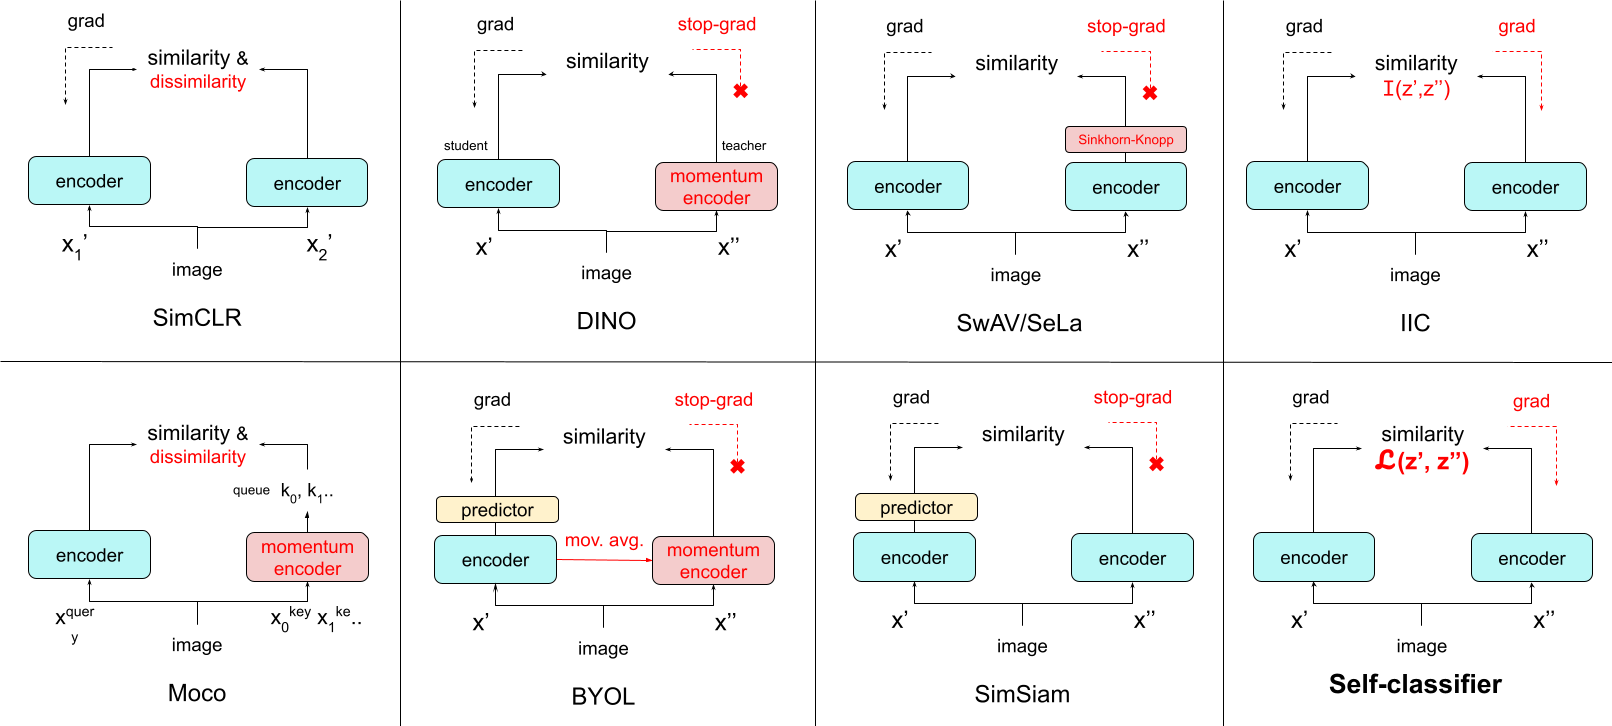
\includegraphics[width=\textwidth]{images/siamese_network_comparison.png}
     \caption{\textbf{Comparison of models on Siamese architectures.} The figure is inspired by the one in SimSiam \cite{simsiam}. We extend it with the main models described in this report. The difference between each model is highlighted in red and represents how the model solves the degenerate problem. The label "dissimilarity" indicates that the model employs negative pairs for training. The dash lines ending with an "X" indicate the presence of a stop gradient operation. The architecture for Self-Classifier is on the bottom right, which is similar to the one proposed in ICC \cite{iic} as they are both based on defining a non-degenerate function.}
    \label{fig:1}
\end{figure}

\subsection{Loss function}
The derivation, the mathematical properties, and the proofs behind the loss function implemented by Self-Classifier are clearly described in the original paper \cite{self_classifier}. In short, the model adopts Bayes and total probability laws on each term of naive cross entropy and assumes a uniform prior for the class probability $p(y)$, providing a mathematical guarantee for the non-degenerate solution. The overall function can be represented as follow:

\[ 
\begin{array}{cc} 
    l(x_1, x_2) = \sum_{y \in [C]} \frac{p(x_2 | y)}{\sum_{\tilde{y}} p(x_2 | \tilde{y})} \log \left( \frac{N}{C} \frac{p(y | x_1)}{\sum_{\tilde{x}_1} p(y | \tilde{x}_1)} \right)
    &
    \mathcal{L} = \frac{1}{2} \Big( l(x_1, x_2) + l(x_2, x_1) \Big)
\end{array}
 \]


\subsection{Implementation Details}
\label{subsec:implementation_details}

\paragraph{Architecture}
Our architecture follows the same as described in the original paper \cite{self_classifier}, with the base architecture of Siamese network \cite{siamese_network}. The model consists of a backbone, followed by a 2-layer MLP with batch normalization and LeakyReLU. A final layer of multiple classification heads is attached to the end. 
Differently from the original paper, we use Resnet-18 instead of Resnet-50 \cite{resnet} to lower the computational cost and adapt to smaller datasets. 
We also scaled down the size of the final classification heads to be proportional to the number of classes in the datasets, keeping the ratio equal to the original paper's.

\paragraph{Image Augmentation}
We use the same augmentations presented in BYOL \cite{byol}, which in turn took them from SimCLR \cite{simclr}\cite{byol}. These augmentations are almost standard in contrastive learning for visual representation and they are used by most of the models we see.
The first augmentation consists in taking a random patch of the image and resizing it. In our implementation, the new dimensions depend on the dataset used. After this, we apply random horizontal flip, color distortion, Gaussian blur, and solarization \cite{byol}. The paper also lists two other augmentations: multi-crop from \cite{swav} and nearest neighbor from \cite{nn_augmentation}. In our model, we skip the nearest neighbor augmentation for simplicity.

\paragraph{Optimization} \quad

\textit{Unsupervised training:} We use a batch size of 512 with softmax temperatures of 0.1 row-wise (over all classes) and 0.05 column-wise (over all batches). We train the model with the SGD optimizer with a 0.9 momentum and 0.0001 weight decay. The learning rate starts at 0.01 and increased linearly to 0.4 within the first 10 epochs. After that, it decreases according to a cosine scheduler over the remaining 790 epochs, reaching a final value of 0.0004.

\textit{Linear training:} We use a batch size of 512. We train the model with the AdamW optimizer with a momentum of 0.9 and no weight decay. The learning rate starts at 0.0004 and decreases toward zero following a cosine scheduler over the 100 epochs of training.

Note that we implemented LARS optimizer as the paper suggested, but it turned out to be worse than AdamW and SGD, which, according to \cite{simsiam}, can be because that LARS is supposed to work better with large batch sizes, not applicable with our limited computation resources.

\section{Data and benchmarks}
\label{sec:data}
%Describe the data you are working with for your project. What type of data is it? Where did it come from? How much data are you working with? Did you have to do any preprocessing, filtering, or other special treatment to use this data in your project? If you are using a very standard dataset (Cifar10 etc) then you should focus on describing the state-of-the-art performing methods on the dataset.

We trained our model on common datasets and compared the obtained results with the standard unsupervised clustering benchmarks publicly available. These are: CIFAR-10 \cite{cifar_10}\footnote{https://paperswithcode.com/sota/image-clustering-on-cifar-10}, CIFAR-20\cite{cifar_100}\footnote{https://paperswithcode.com/sota/unsupervised-image-classification-on-cifar-20}, STL-10 \cite{stl_10} \footnote{https://paperswithcode.com/sota/image-clustering-on-stl-10} and MNIST \cite{mnist}\footnote{https://paperswithcode.com/sota/image-clustering-on-mnist-full}. 

\section{Experiments and findings}
\label{sec:results}
%Describe and present the experiments that you performed in detail and what is the reason for those experiments. Where applicable define evaluation metrics that you used. Discuss the results that you got. You should include graphs, tables, or other figures to illustrate your experimental results. This is the most important part of your report, be thorough, clear and detailed. Does the reporduction show a significant deviation from those results reported in the original paper? What could be the reason? What extra experiments can you think of to substantiate those speculated reasons? Do the conclusions, observations, statements, and theories of the original paper hold in the new experiments or datasets that you have tried? To what extent? Discuss the similarities and discrepancies and the possible reasonings. 
\subsection{Clustering results}
We report the results based on standard clustering evaluation metrics illustrated in \autoref{tab:results}. The numbers are sub-optimal compared to the state-of-the-art methods in the unsupervised clustering benchmarks but achieve substantial improvement over the earlier methods. Although part of the reason for the unsatisfactory result may be that the hyperparameters are not tuned to the best, we also inferred that it could be because the method does not fit well in smaller datasets with low-resolution image inputs, i.e. the prior enforcement of the loss function requires abundant unseen data while none of the datasets we adopted can provide. The difference in the number of classes could also be a contributing factor. Further analysis on middle and large datasets needs to be run in order to explain the performance drop here.

\begin{table}[h!]
  \caption{\textbf{Unsupervised image clustering using ResNet-18.} NMI: Normalized Mutual Information, AMI: Adjusted Normalized Mutual Information, ARI: Adjusted Rand-Index, ACC: Clustering accuracy. The performance falls behind SOTA models but is competitive compared to earlier models. The results are aligned with the difficulty of each benchmark, somewhat validating our implantation.}
  \label{tab:results}
  \centering
  \begin{tabular}{lcccc}
    \toprule
    Dataset  & NMI    &  AMI     & ARI   & ACC  \\
    \midrule
    MNIST\cite{mnist}   & 83.9427 & 83.9140 & 76.8142 & 81.9000 \\
    CIFAR-10 \cite{cifar_10} & 50.9317 & 50.8450 & 41.5156 & 60.7300 \\
    CIFAR-20 \cite{cifar_100} & 30.9210 & 30.4974 & 17.8501 & 32.2400 \\
    STL-10 \cite{stl_10}  & 42.5199 & 42.3921 & 31.6741 & 51.8125	\\
    \bottomrule
  \end{tabular}
\end{table}

\subsection{Linear probing}
Following the linear classification protocol introduced in the original article, we froze the backbone parameters of the model after the unsupervised training and replaced the MLP and head layers with a single linear layer for a 100-epoch supervised training using standard cross-entropy loss. \autoref{fig:linear} reports Top-1 and Top-3 accuracy for the classification performance. It is clearly shown in the figure that the quality of representations learned by the model improves with the number of epochs and the linear model converges to a satisfactory state at approximately epoch 500. The results of this experiment are compatible with those of unsupervised clustering, which validates the fact that the model simultaneously improves representation learning and clustering performance.


\subsection{Qualitative results}
% Paper says: Visualization of High/Low Accuracy Classes Predicted by Self-Classifier
\paragraph{Cluster images visualization} 
Following the paper, we report image samples of clusters with high and low accuracy from different datasets.
As observed in \autoref{fig:visualization}, the displayed images for each assigned cluster show strong consistency in the semantic meaning which validates the success of our implementation. While it is harder to identify miss-classified samples from STL-10 \cite{stl_10}, due to its competitive clustering performance the representations in CIFAR-20 contain more errors. Specifically, \autoref{fig:low_cifar20} shows images of $fox$ and $squirrel$ clustered together, while they belong to separate classes, $medium-sized\ mammals$ and $small\ mammals$ respectively.
% I would say: Not a big deal... But we can leave it as it is

\begin{figure}[hbt!]
     \centering
     \begin{subfigure}[b]{.45\textwidth}
         \centering
         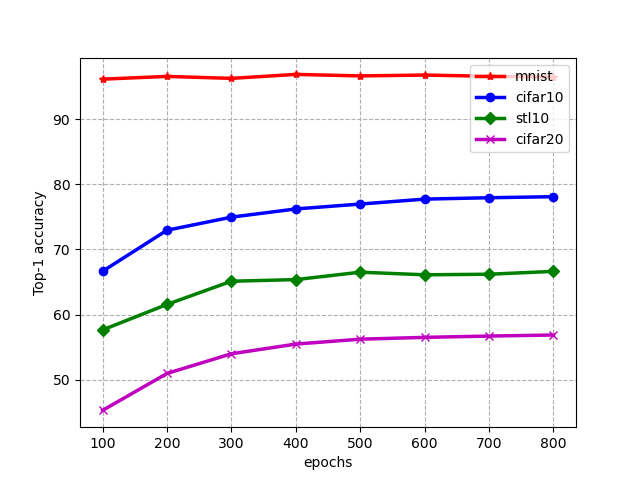
\includegraphics[width=\textwidth]{images/linear_probing_top1.png}
         \caption{Top-1 Accuracy}
         \label{fig:top1}
     \end{subfigure}
     \hfill
     \begin{subfigure}[b]{0.45\textwidth}
         \centering
         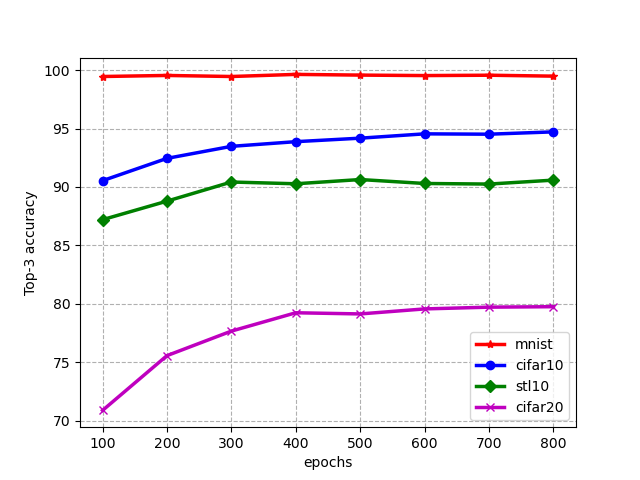
\includegraphics[width=\textwidth]{images/linear_probing_top3.png}
         \caption{Top-3 Accuracy}
         \label{fig:top3}
     \end{subfigure}
     \caption{\textbf{Linear probing.} The x-axis indicates the pre-trained epochs of unsupervised learning before linear probing while y-axis represents the supervised performance.}
     \label{fig:linear}
\end{figure}

\begin{figure}[hbt]
     \centering
     \begin{subfigure}[b]{0.48\textwidth}
         \centering
         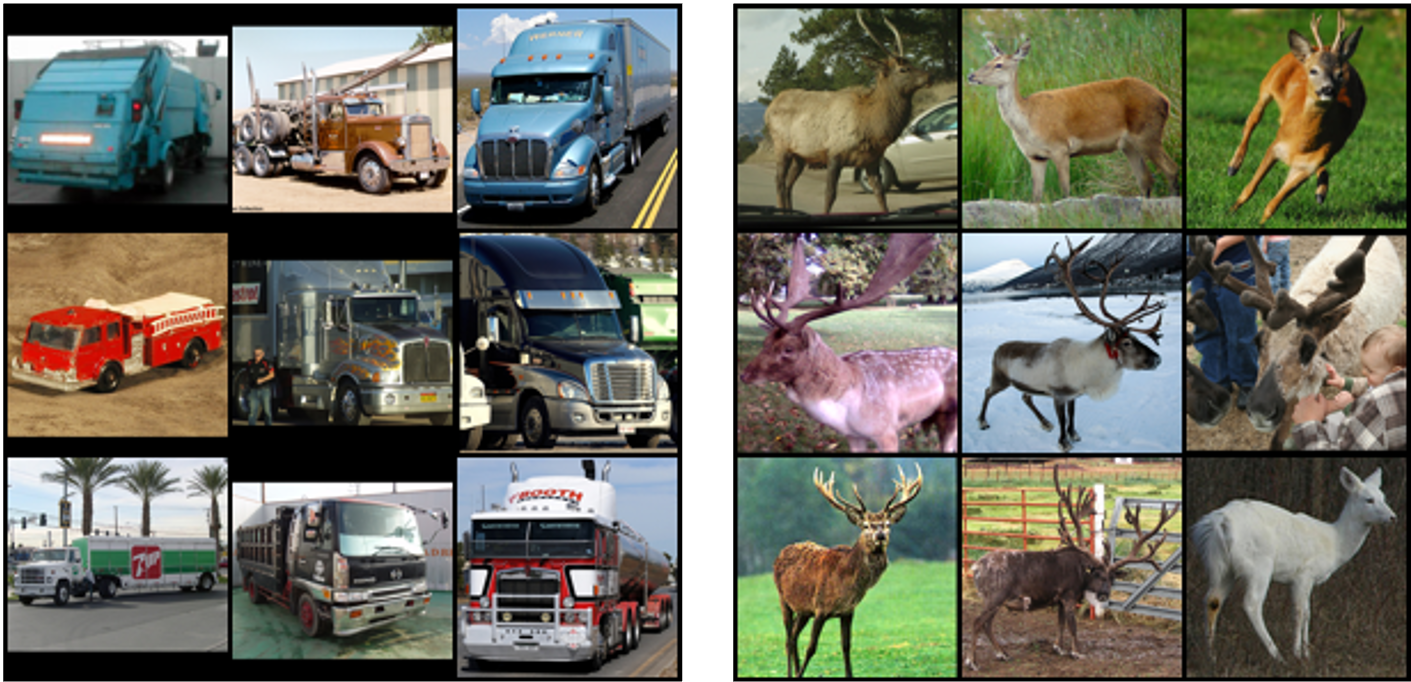
\includegraphics[width=\textwidth]{images/high_accuracy_stl10.png}
         \caption{High accuracy clusters in STL-10}
         \label{fig:high_stl10}
     \end{subfigure}
     \hfill
     \begin{subfigure}[b]{0.48\textwidth}
         \centering
         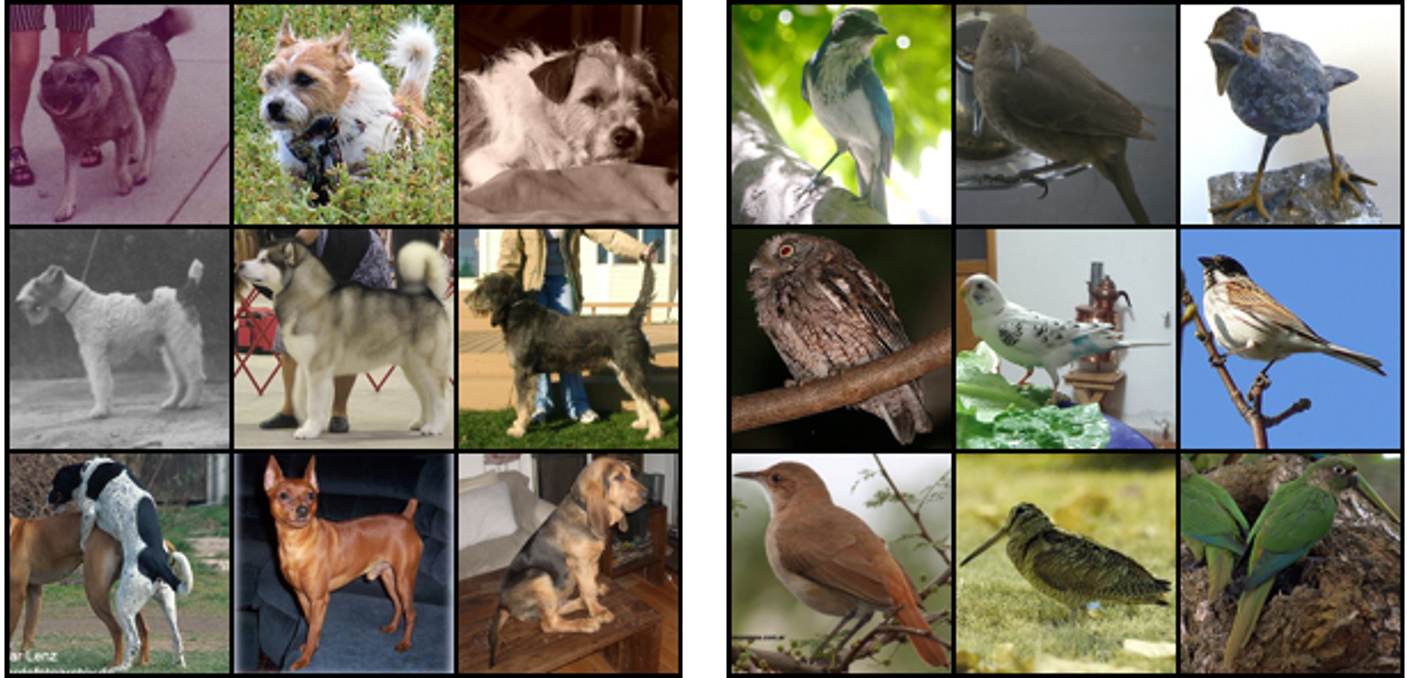
\includegraphics[width=\textwidth]{images/low_accuracy_stl10.png}
         \caption{Low accuracy clusters in STL-10}
         \label{fig:low_stl10}
     \end{subfigure}
     
     \begin{subfigure}[b]{0.48\textwidth}
         \centering
         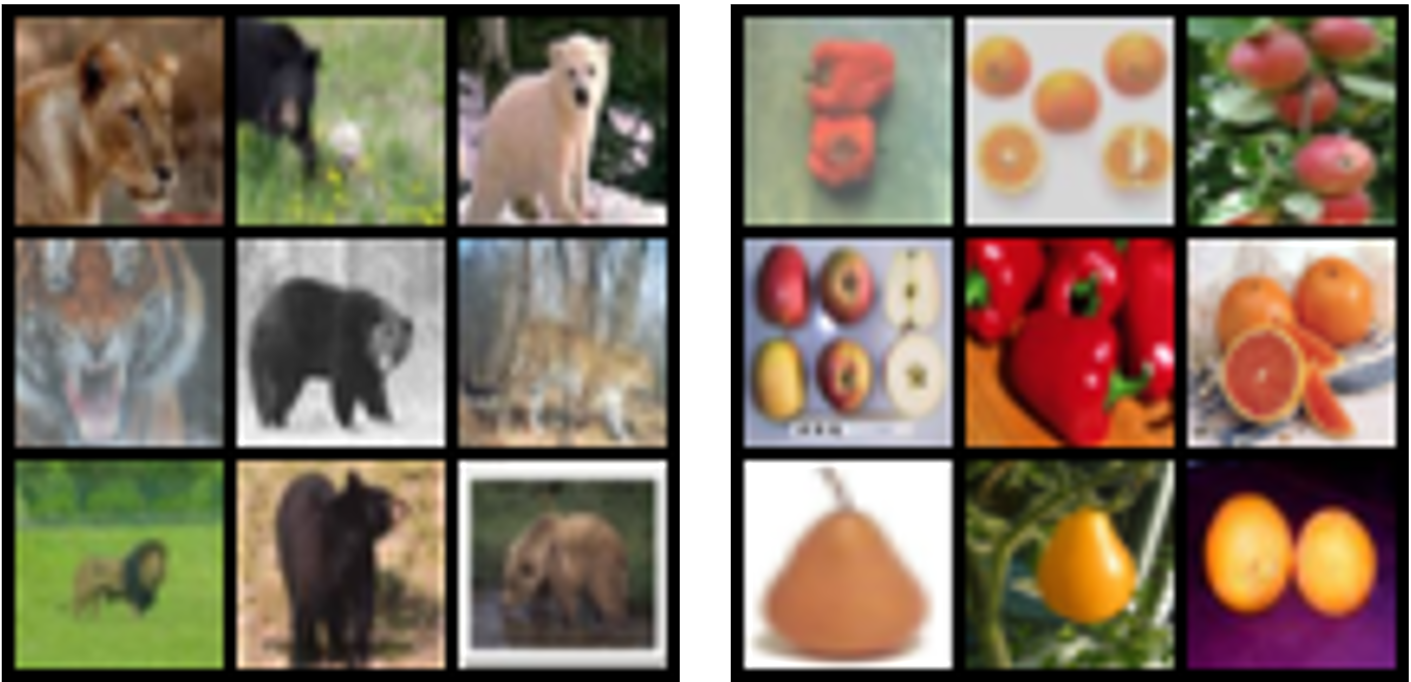
\includegraphics[width=\textwidth]{images/high_accuracy_cifar20.png}
         \caption{High accuracy clusters in CIFAR-20}
         \label{fig:high_cifar20}
     \end{subfigure}
     \hfill
     \begin{subfigure}[b]{0.48\textwidth}
         \centering
         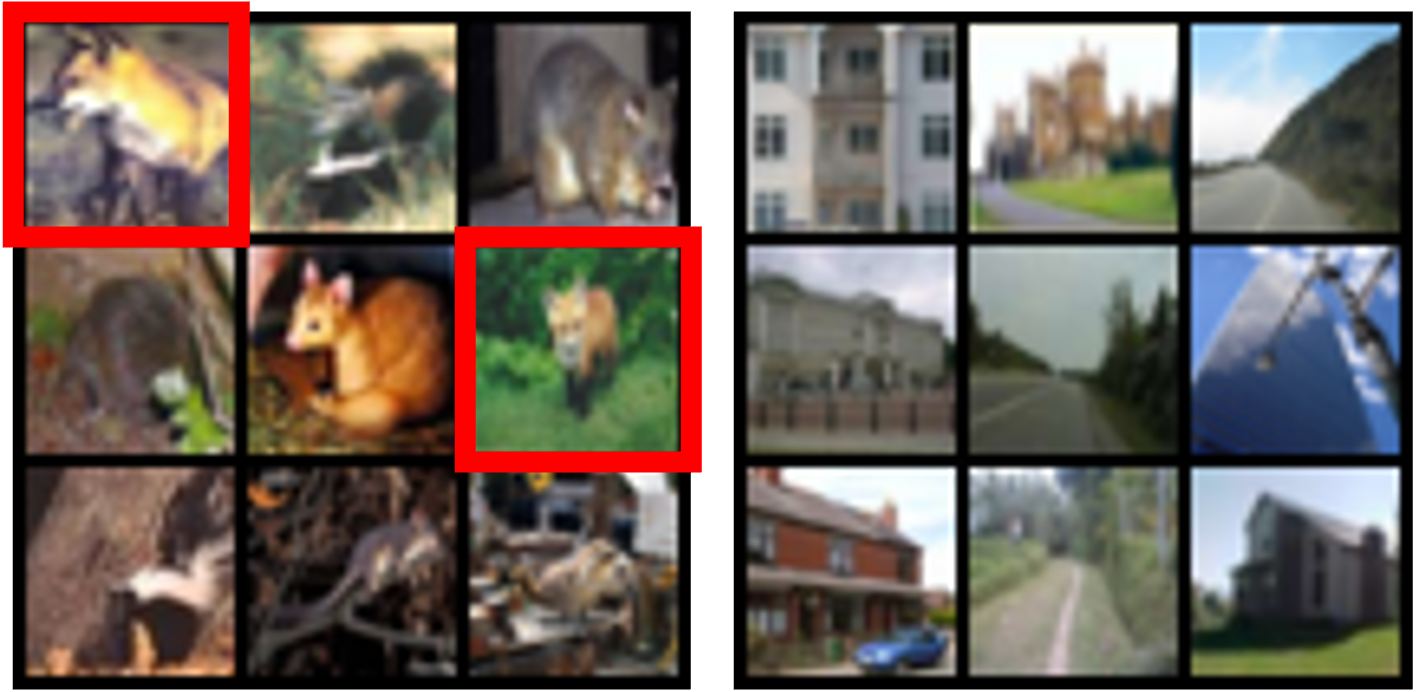
\includegraphics[width=\textwidth]{images/low_accuracy_cifar20.png}
         \caption{Low accuracy clusters in CIFAR-20}
         \label{fig:low_cifar20}
     \end{subfigure}
     \caption{\textbf{Image visualization for high and low accuracy classes in different datasets.}}
     \label{fig:visualization}
\end{figure}
\begin{figure}[hbt!]
     \centering
     \begin{subfigure}[b]{0.45\textwidth}
         \centering
         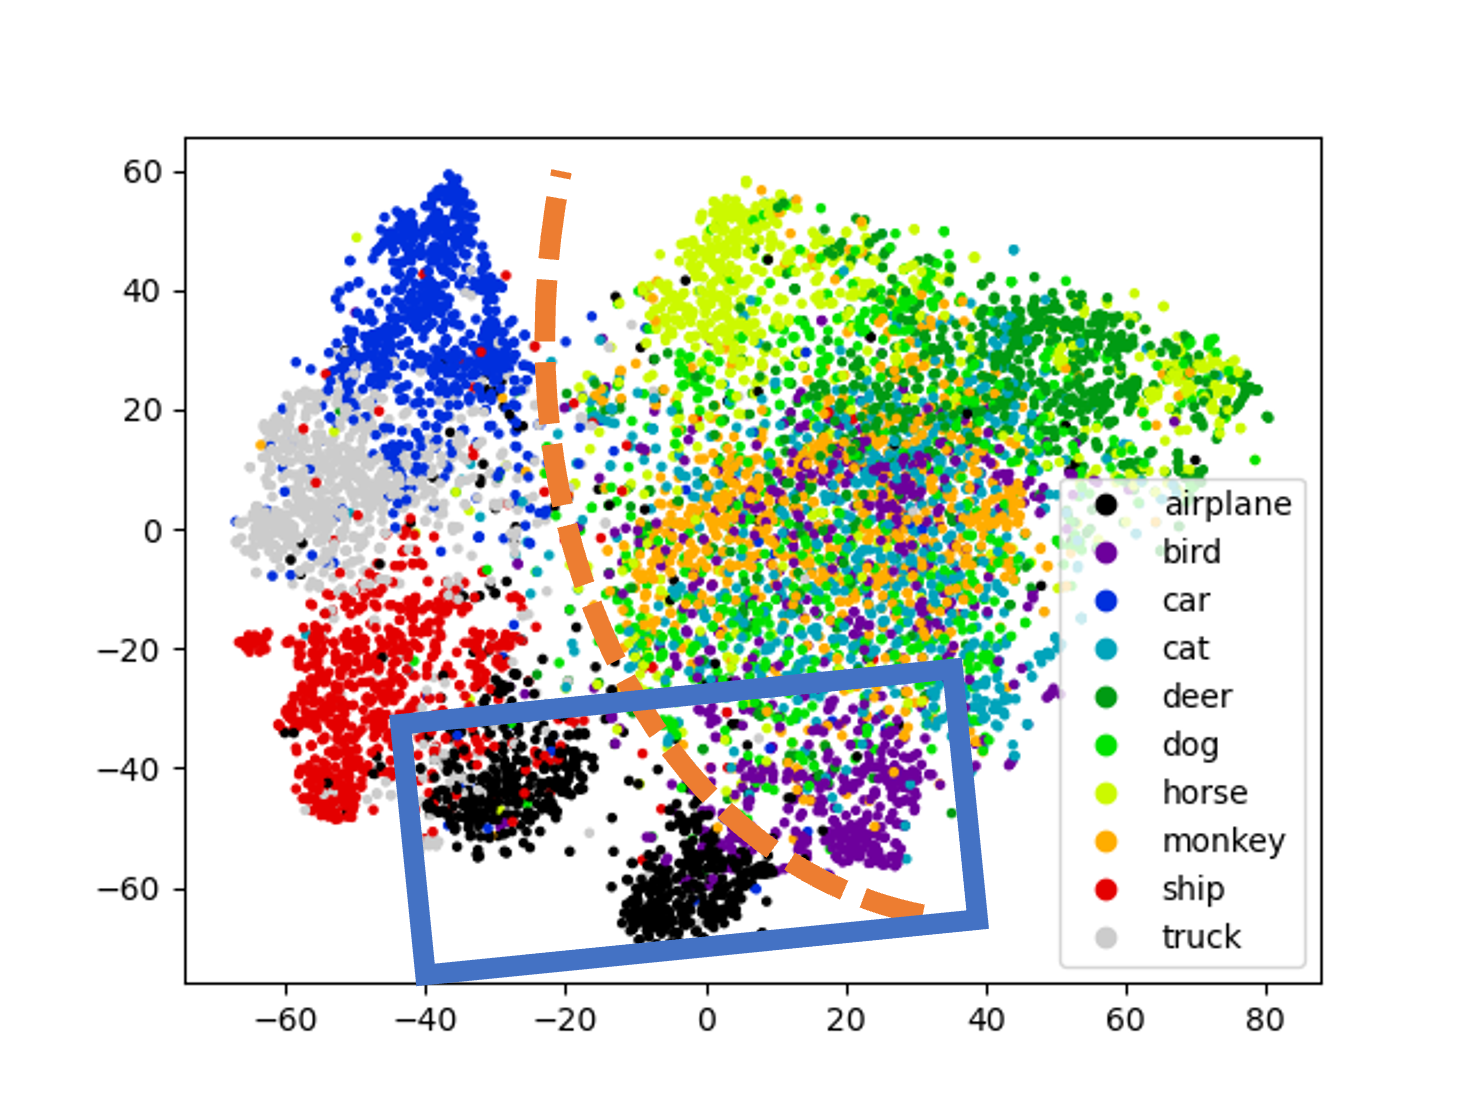
\includegraphics[width=\textwidth]{images/stl10_tsne.png}
         \caption{T-SNE feature visualization.}
         \label{fig:t_sne}
     \end{subfigure}
     \hfill
     \begin{subfigure}[b]{0.45\textwidth}
         \centering
         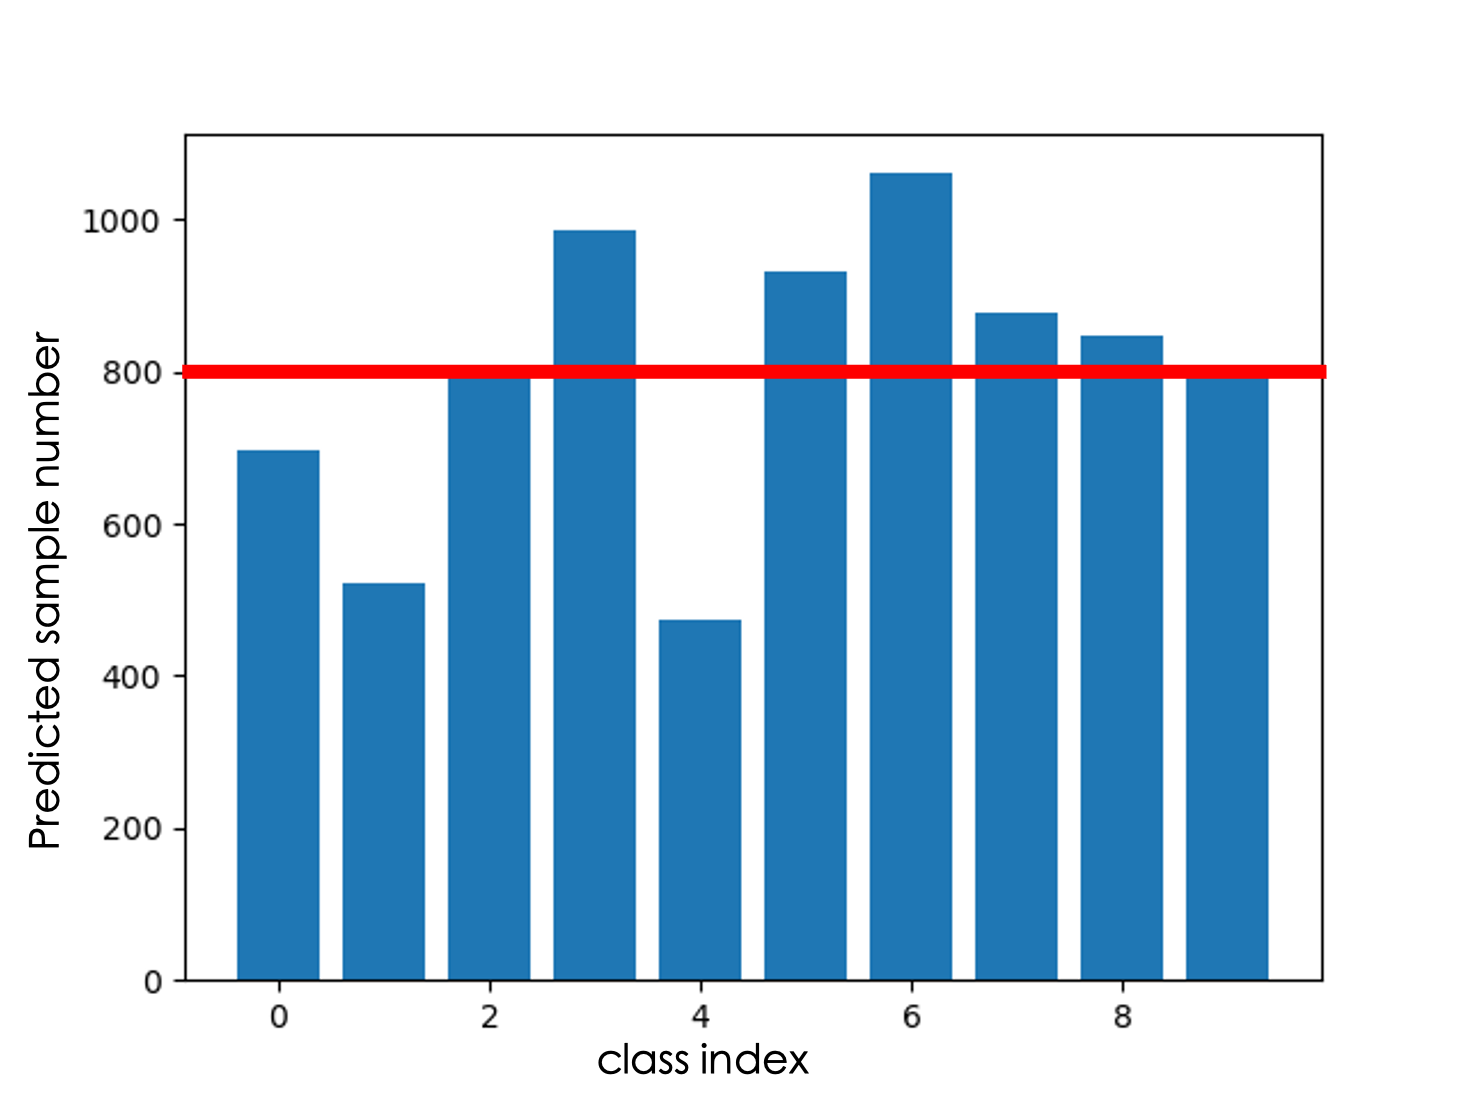
\includegraphics[width=\textwidth]{images/stl10.png}
         \caption{Predicted class number}
         \label{fig:distribution}
     \end{subfigure}
     \caption{\textbf{Additional visualization on dataset STL-10.} In subfigure (a), the orange dotted line separates human artifacts from natural animal features, and the blue square indicates the similarity between birds and airplanes; In subfigure (b), the red line is the actual class number (800 samples)}
     \label{fig:combine}
\end{figure}

\paragraph{Additional visualization with t-SNE and predicted class number}
We also ran additional feature visualization over the model trained on STL-10 using t-SNE shown in \autoref{fig:t_sne}. Interesting insights can be concluded from the figure including 1) There is a noticeable separation between natural classes ($cat, dog...$) displayed on the right side of the figure and artifact classes ($car, airplane$) on the left side. 2) Aside from inner-class consistency, the figure also demonstrates inter-class connection regarding their similarity $e.g.$ $bird$ and $airplane$ class stay rather close at the bottom. Overall the result confirms how well the model learns to distinguish the different classes by extrapolating their main features. We would like to ensure the uniform prior distribution is well enforced through the model training, so we visualized the sample number over each predicted class in\autoref{fig:distribution}. While the numbers of each class are not exactly the same, the degenerate solution is clearly avoided with the proposed loss function.

\subsection{Ablation Study}

We focus the ablation studies on the STL-10 \cite{stl_10} dataset. \autoref{tab:ablation} shows comparisons between the base model and its variants, which are different in batch sizes, classification head sizes, temperature settings, or multi-crop augmentation usage. As in \cite{byol}, we trained the model for 300 epochs for each configuration, as fewer iterations may not guarantee stable behavior. We can state that Self-Classifier is somewhat robust to different hyperparameter settings, with performance fluctuations under $5\%$ for NMI and $8\%$ for ACC. We assume ACC is more subject to oscillations because of the second step (linear sum assignment) adopted for unsupervised accuracy calculation. Interestingly, larger batches and more heads do not necessarily lead to better results. The numbers show a $1-4\%$ decrease in the accuracy when using the largest batch size compared to the smallest, which is quite counterintuitive. We assume that, while the loss function expects a larger batch size to enforce the uniform priors, a smaller batch size brings more randomness in the optimization resulting in a trade-off between the two above properties. Also, the performance drop brought by the additional multi-crop augmentation can be explained by the small resolution of images causing the local patches (even smaller) with limited knowledge to aid the entire training process.

\begin{table}[htb!]
  \caption{\textbf{Ablation study on unsupervised clustering metrics.} The base model has 512 batch size, $[10,20,40,80]$ classification head size, and (0.10, 0.05) temperature setting.}
  % The model is not sensitive to hyperparameter settings in general.
  \label{tab:ablation}
  \centering
  \begin{tabular}{clcccc}
    \toprule
    \multicolumn{2}{c}{Model Variants} & NMI &  AMI & ARI & ACC  \\
    \midrule
    \multirow{3}{*}{Batch Size} & 128 & 39.0715 & 38.9363 & 27.6416 & 48.8500\\
    & 256 & 41.0984 & 40.9675 & 27.3900 & 46.4750\\
    & 1024 & 39.6265 & 39.4921 & 26.2468 & 45.2375 \\
    \midrule
    \multirow{4}{*}{Head Size} & $1*10$ & 39.8843 & 39.7506 &  27.4368 & 48.7750 \\
    & $5*10$  & 38.2264 & 38.0888 & 26.1061 & 47.3250 \\
    & $10*10$ & 38.8565 & 38.7202 & 25.2499 & 44.5375 \\
    & $15*10$ & 39.9663 & 39.8326 & 25.9415 & 44.0750 \\
    \midrule
    \multirow{3}{*}{\shortstack{Temperature\\$(\tau_{row}, \tau_{col})$}} & $(0.07, 0.03)$ & 40.8495 & 40.7174 & 28.4016 & 48.4375 \\
    &$(0.07, 0.05)$ & \textbf{42.5199} & \textbf{42.3921} & \textbf{31.6741} &  \textbf{51.8125}	 \\
    &$(0.10, 0.03)$ & 40.6805 & 40.5485 & 27.7525 & 45.7875 \\
    \midrule
    \multicolumn{2}{c}{Base with Multi-Crop} & 40.5333 & 40.4014 & 25.5025 & 45.0875\\
    \multicolumn{2}{c}{Base} & 40.3517 & 40.2191 & 29.2059 & 50.3375\\
    \bottomrule
  \end{tabular}
\end{table}
    
\section{Challenges}
\label{sec:challenges}
%Challenges you faced when reimplmenting the paper and conducting the experiments. Were all details in the paper? Or did you have to look in the authors code or contact authors to find about some details (you are encouraged to contact the authors)? Was parts of the code quite hard to get them to work as intended? Did you have optimize and tune several hyperparameters? Which ones? Did the framework you used  make the implementation difficult in some ways? 
The main challenge that occurred in the implementation is to check for the specific values of some of the hyperparameters in the official repository (e.g. optimizer and augmentation specifics like kernel size for the Gaussian blur) 
Even with reference to the official code, we did not implement the nearest neighbor augmentation mentioned in the paper for its significant increase in computational cost, and the improvement is rather not obvious. 
Also, we spent a lot of time tuning the hyperparameters like which optimizer to choose, the batch size, learning rate, etc. with some of the results included in the ablation study. Also, we noticed an interesting thing that sometimes a minor modification in learning rate (0.04 to 0.05 for example) could cause a significant increase or drop in performance.

    
\section{Conclusion}
\label{sec:conclusion}
%Summarize your key results - what have you learned? What points do you think one should consider when using the approach of the paper you chose for your project? What can go wrong when reimplementing based on paper and why? A summary of similarities and discrepancies that you found when conducting the experiments. Suggest ideas for future extensions or new applications of your ideas.
In this work, we successfully re-implement Self-Classifier \cite{self_classifier} and explained in detail the peculiarities it has compared to other models designed to solve the degenerate solution problem and why it is revolutionary. We then demonstrate its capabilities to achieve comparable results on multiple smaller datasets and how it simultaneously solves the feature representation and clustering tasks through both quantitative experiments and extensive visualizations, which suggest that the model may be more suitable in larger datasets. Overall, most of the obtained results are in alignment with the paper suggested, but we do fall behind the intended SOTA performance. If our work is correct then future work could be done to improve the model's performance on smaller datasets and try to reduce its reliance on a known class number, for that can sometimes be hard to obtain.

% The only thing we can not express our argument on is the performance of the model in the new hierarchical alignment metric the paper introduced, as we did not define it for the smaller datasets we used.

% \section{Ethical consideration, societal impact, alignment with UN SDG targets}
%Think and research! Are there any ethical considerations for the original paper, its problem or method, its way of conducting experiments? How about the experiments you did? What societal impact can you imagine about the original paper and its contributions and results? How about your project report? How do you think this paper can push or inhibit the UN SDG targets?

\section{Self Assessment}
%Use the Project Grading Guideline again and assess your project along those guidelines. Argue what grade you think your project deserves and why.

Overall, we did comprehensive and concrete experiments over our implemented model, with some evaluation metrics going beyond the original paper's. We have put a lot of effort into report writing, clearly addressed interesting findings during the implementation as well as summarized the previous literature with detail and our own opinions. We believe this to be in line with the assessment criteria for the grade "very good" or "excellent".


\medskip

\small
\bibliographystyle{plain}
\bibliography{report.bib}

\end{document}
